We now introduce a mechanical degree of freedom into our optical system and thereby realizing  an optomechanical system. In our case we will allow for the end mirror to move, for example like a harmonic oscillator, see figure \ref{fig:E-field_model_moving}. These kinds of systems come in many various constellations, e.g. microtoriods \cite{weis2010} and the photonic crystal nano beam \cite{chan2011}. Both of these systems have produced great results, such as ground state cooling and and optomechanical induced transparency. For an extended overview of different systems see \cite{aspelmeyer2014}.

\begin{figure}[H]
\centering
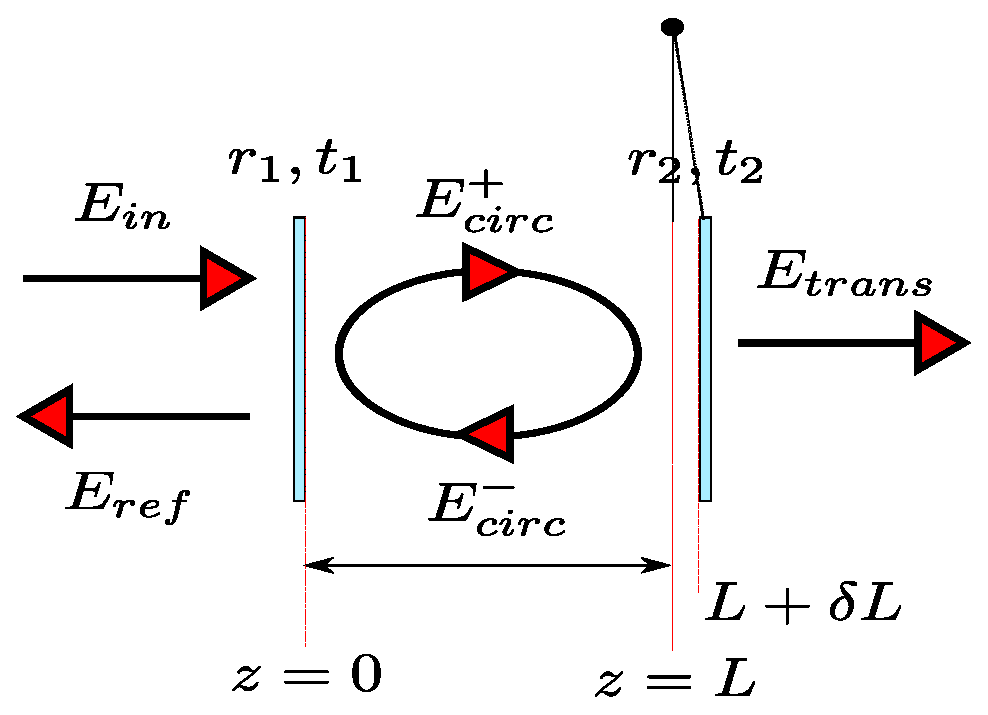
\includegraphics[scale=0.8]{E-field_model.eps}
\caption{We allow for a small pertubation to the cavity length $\delta L$. Here the mechanical degree of freedom is the not canonical pendulum, for visual purposes. The cannonical}
\label{fig:E-field_model_moving}
\end{figure}

We want to investigate the effect of a movable end mirror in a cavity. We introduce a displacement of the end mirror as a small perturbation $\delta L$ to the otherwise fixed cavity length $\tilde{L} = L + \delta L$ and assume that $\delta L \ll L$. The perturbation changes our cavity resonance frequency $\omega_c \rightarrow \omega_c^\prime$.

\begin{equation}
\omega_c^\prime = 2\pi\frac{c}{2\left( L + \delta L \right)}n
\end{equation}
\noindent
a linearization of the equation above yields

\begin{equation}
\omega_c^\prime \approx \omega_c - \frac{\omega_c}{L}\delta L
\label{eq:opt_coup}
\end{equation}
\noindent
This result is for the special case of a Fabry-Perot cavity. A more general way of writing the mechanical induced modulation of the cavity resonance would be, again only keeping the linear term

\begin{equation}
\omega_c^\prime(z) \approx \omega_c + \delta z\frac{\partial\omega_c}{\partial z}\bigg|_{z = z_0}
\end{equation}
\noindent
We normally define the optical frequency shift per displacement as $G \equiv \left|\frac{\partial\omega_c}{\partial z}\right|$. We easily recognize that for a Fabry-Perot cavity it is just the cavity resonance divided by the cavity length $G_{FP} = \frac{\omega_c}{L}$ as seen in equation \eqref{eq:opt_coup}. Note that $G_{FP}$ is inversely proportional to the cavity length $L$, so smaller cavity length are preferred.

We deliberately avoided using the term ``optomechanical coupling" in this section, since it is the cause of confusion in this field of study\footnote{Do not say I did not warn you!}.